\section{Der Algorithmus}

Wie in der Einleitung schon erw"ahnt worden ist, arbeitet der Simplex-Downhill
Algorithmus ohne Ableitungen.

Warum das funktioniert wird klar, wenn man sich vorstellt, dass das
Simplex selber auf der Zielfunktion liegt und sozusagen die Ableitung
approximiert. Sucht der Algorithmus ein Minimum, so bewegt er sich
nat"urlich abw"arts (downhill), was auch seine Namensgebung erkl"art.
Der Algorithmus ist ebenfalls in der Lage nach Maxima zu suchen, indem
die Zielfunktion einfach invertiert wird.

Im Folgenden wird immer davon ausgegangen, dass ein Minimum gesucht wird.

\subsection{Hauptablauf}
Der Algorithmus besteht aus einer Initialisierung, einer
Iterationsschlaufe und einer Abbruchbedingung (siehe
\figref{fig:downhillalgo1})

\begin{figure}[h]
\resizebox{1\textwidth}{!}{
\providecommand{\highlight}{white}
\begin{tikzpicture}[node distance = 1.7cm,every node/.style={rectangle,fill=white},
  block/.style={draw,align=center},
  highlight/.style={draw,fill=\highlight},
  line/.style = {draw,-latex'}
]

\node (start) [block] {N+1 Startpunkte $x_i$ w"ahlen (Simplex bilden)};

\node (a1) [block, below of=start] { $y_i = f(x_i)$ berechnen};

\node (a2) [block, below of=a1] { Bestes ($y_{min}$) und schlechtestes ($y_{max}$) $y_i$ bestimmen};

\node (a3) [block, below of=a2,text width=5cm]{Abbruchbedingung erf"ullt?};

\node (ende) [block, below of=a3] {Ende};

\node (a4) [highlight, left of=a3, node distance=6cm] {Neuer Simplex bilden};



\path[line] (start) -- (a1);
\path[line] (a1) -> (a2);
\path[line] (a2) -> (a3);

\path[line] (a3) -> node{ja} (ende);
\path[line] (a3) -> node{nein} (a4);

\path[line] (a4)  |-  (a1.west);

\end{tikzpicture}
}

\caption{"Ubersicht des Algorithmus}
\label{fig:downhillalgo1}
\end{figure}

\begin{itemize}
\item
Zu Beginn wird ein Simplex mit den Ecken $x_i$ gebildet.
\item
Zu den gew"ahlten $x_i$ werden nun die dazu geh"origen $y_i$ der
Zielfunktion ausgerechnet.
\item
Aus den erhaltenen Funktionswerten wird der beste $y_{min}$, der
schlechteste $y_{max}$ sowie der Mittelwert ohne $x_{max}$ extrahiert.
Diese werden f"ur die Abbruchbedingung \chapref{sec:downhillAbbruch}
und zur Bildung des neuen Simplex ben"otigt, siehe
\chapref{sec:downhillModi}.
\item
Hat man das Simplex auf der Zielfunktion platziert, werden die
berechneten
Testpunkte gepr"uft, wobei der schlechteste dieser Punkte mittels
gewisser ''Taktiken`` ersetzt wird.
\item
Dies wird solange fortgef"uhrt, bis
das gew"unschte Ergebnis erreicht worden ist bzw. eine Abbruchbedingung
erf"ullt ist.
\end{itemize}

\subsection{Abbruchbedingungen}
\label{sec:downhillAbbruch}
Es k"onnen diverse Abbruchbedingungen f"ur den Downhill-Simplex verwendet werden:
\begin{itemize}
\item Der Wert von $y_{min}$: Es kann abgebrochen werden, sobald ein gewisser Wert unterschritten wird.
\item Werte von $x_i$: Sobald alle $x_i$ nahe beieinander sind, wird abgebrochen, da es keine grosse "Anderung mehr gibt.
\item Maximale Iterationszahl: Als Notfall wenn nicht konvergiert wird.
\end{itemize}

Es empfiehlt sich eine Kombination der Abbruchbedingungen, um die
Iterationszahl m"og\-lichst gering zu halten.


Im Allgemeinen ist es ratsam, die $x_i$ und Anzahl Iterationen zu
verwenden, da so kein Wissen "uber die Art des Minimums der Zielfunktion
ben"otigt wird.
Ist die gew"ahlte Abbruchbedingung erf"ullt, ist der Algorithmus am Ende.
Es ist nat"urlich eher Zufall, wenn man gleich bei der ersten
Wahl des Simplex das Minimum trifft, meistens hat man es nicht
getroffen und es wird nun auf Grund des gew"ahlten Simplex gem"ass
\chapref{sec:downhillModi} ein neues Simplex gebildet.

\subsection{Neuen Simplex bilden}
\label{sec:downhillModi}

Das Auswahlverfahren des neuen Simplex unterliegt einer Reihe von
Faktoren. Die Entscheidungen werden vor allem aufgrund der gegebenen
Eckpunkte sowie deren Funktionswerte getroffen.
In \figref{fig:downhillalg2} ist dieser Entscheidungsbaum ersichtlich.

\begin{figure}[h]
\resizebox{1\textwidth}{!}{
\providecommand{\highlightref}{white}
\providecommand{\highlightexp}{white}
\providecommand{\highlightrefb}{white}
\providecommand{\highlightcona}{white}
\providecommand{\highlightconb}{white}
\providecommand{\highlightkomp}{white}
\usetikzlibrary{shapes}
\begin{tikzpicture}[
  node distance=2.2cm,
 every node/.style={rectangle,fill=white},
  hlref/.style={draw,align=center,text width=5cm,  fill=\highlightref},
  hlexp/.style={draw,align=center,text width=5cm,  fill=\highlightexp},
  hlrefb/.style={draw,align=center,text width=5cm, fill=\highlightrefb},
  hlcona/.style={draw,align=center,text width=5cm, fill=\highlightcona},
  hlconb/.style={draw,align=center,text width=5cm, fill=\highlightconb},
  hlkomp/.style={rounded corners, draw,align=center,text width=5cm, fill=\highlightkomp},
  med/.style={draw,align=center,text width=5cm},
  fin/.style={rounded corners,draw,align=center, text width=5cm},
  line/.style = {draw,-latex'}
]

\tikzstyle{level 1}=[sibling distance=100mm,align=center]
\tikzstyle{level 2}=[sibling distance=100mm,align=center]
\tikzstyle{level 3}=[sibling distance=80mm]


\node (spiegeln) [hlref] {$x_{max}$ am Mittelpunkt des restlichen Simplex ($x_m$) spiegeln $\rightarrow$ $x_{ref} = x_m + \alpha(x_m-x_{max})$};

\node[med, below of=spiegeln](spiegelnq){$y_{ref}$ besser als  $y_{min}$?};
\node[hlexp, below of=spiegelnq](streck) {Expansion: In Richtung $x_{ref}$ mit Faktor $\gamma$ Strecken  $\rightarrow x_{streck} = x_{ref} + \gamma (x_{ref} - x_m)$};
\node[med, below of=streck](streckq)  {$y_{streck}$ besser als $y_{min}$?};

\node [below of=streckq](split1){};
\node[med,below of=streckq](expansion){$x_{max}$ mit $x_{streck}$ ersetzen};
\node[fin, right of = expansion,node distance=6.6cm](reflektion){$x_{max}$ mit $x_{ref}$ ersetzen};

\path[line] (spiegeln) -- (spiegelnq);
\path[line] (spiegelnq) -> node{ja} (streck);
\path[line] (streck) -- (streckq);
\path[line] (streckq) -> node{ja} (expansion);
\path[line] (streckq) -> node{nein} (reflektion);


\node [hlrefb,right of=spiegelnq, node distance=6.6cm](spiegelnq2) {$y_{ref}$ besser als zweitschlechtestes $y_i$ ?};
\path[line] (spiegelnq) -> node{nein} (spiegelnq2);
\path[line] (spiegelnq2) -> node{ja} (reflektion);

\node[med, right of=spiegelnq2, node distance=6.6cm] (kont2q) {Ist $y_{ref}$ besser als $y_{max}$? };
\path[line] (spiegelnq2) -> node{nein} (kont2q);
\node[hlconb, right of=kont2q, node distance=6.6cm] (kont2){Ersetze $x_{max}$ durch $x_{ref}$ };
\path[line] (kont2q) -> node{ja} (kont2);

\node[hlcona, below of=kont2q] (kont){Kontraktion: R"ucke mit Faktor $\beta$ n"aher an $x_m$ $\rightarrow x_{kon}$ };
\node[med, below of=kont] (kontq){Ist $y_{kon}$ besser als $y_{max}$?};
\path[line] (kont2q) -> node{nein} (kont);
\path[line] (kont) ->  (kontq);
\path[line] (kont2) |-  (kont);

\node[below of=kontq](split2){};
\node[fin,below of=kontq](kontraktion) {Ersetze $x_{max}$ durch $x_{kon}$};
\node[hlkomp,right of=kontraktion, node distance=6.6cm](komprimierung) {Komprimierung: R"ucke alle $x_i$ zu $x_{min}$ };
\path[line] (kontq) -> node{ja} (kontraktion);
\path[line] (kontq) -> node{nein} (komprimierung);

\end{tikzpicture}
}

\caption{Algorithmus zur Auswahl der Modifikation}
\label{fig:downhillalg2}
\end{figure}

Die M"oglichkeiten das Simplex soweit zu ver"andern, dass es den optimalen
Punkt findet, sind begrenzt.

Die Darstellungen beziehen sich hierbei auf einen Simplex der zweiten
Dimension (Dreieck), nat"urlich gelten diese Modifikationen auch f"ur
einen $n$-dimensionalen Simplex.

\begin{figure}[ht]
	\centering
	\resizebox{0.8\textwidth}{!}{
\definecolor{uuuuuu}{rgb}{0.27,0.27,0.27}
\definecolor{zzttqq}{rgb}{0.6,0.2,0}
\definecolor{qqqqff}{rgb}{0,0,1}
\begin{tikzpicture}[line cap=round,line join=round,>=triangle 45,x=1.0cm,y=1.0cm]
%\clip(4.51,0.05) rectangle (11.48,4.25);
\fill[color=zzttqq,fill=zzttqq,fill opacity=0.1] (5.74,3) -- (10.36,4) -- (11,2) -- cycle;
\draw [color=zzttqq] (5.74,3)-- (10.36,4);
\draw [color=zzttqq] (10.36,4)-- (11,2);
\draw [color=zzttqq] (11,2)-- (5.74,3);
\draw [color=zzttqq] (11,2)-- (5.74,3);
\begin{scriptsize}
\fill [color=qqqqff] (5.74,3) circle (1.5pt);
\draw[color=qqqqff] (5.75,3.11) node {$x_{\text{min}}$};
\fill [color=qqqqff] (10.36,4) circle (1.5pt);
\draw[color=qqqqff] (10.53,4.07) node {$x_{\text{max}}$};
\fill [color=qqqqff] (11,2) circle (1.5pt);
\draw[color=qqqqff] (11.08,2.08) node {$x_3$};
\fill [color=uuuuuu] (8.37,2.5) circle (1.5pt);
\draw[color=uuuuuu] (8.48,2.47) node {$x_m$};
\end{scriptsize}
\end{tikzpicture}
}
%
  	\caption{Simplex im zweidimensionalen Raum}%
	\label{fig:downhillStart}
\end{figure}

Der Algorithmus w"ahlt auf Grund der Werte der Startsimplex (siehe
\figref{fig:downhillStart}) beziehungsweise deren Zielfunktionswerte
die Modifikationsart aus.

\subsubsection{Reflexion}

Zu Beginn wird das Simplex ziemlich grob behandelt, indem man erst einmal
durch Reflexion versucht, weg vom schlechtesten Punkt zu kommen.

Bei der Reflexion wird der schlechteste Punkt $x_{\text{max}}$ am
Schwerpunkt $x_m$ des restlichen Simplex gespiegelt und mit einem Faktor
$\alpha$ gewichtet:

\begin{equation}
x_m = \left(\sum_1^{N+1} x_i - x_{\text{max}}\right) \frac{1}{N} \quad N = \text{Anzahl Dimensionen}
\end{equation}

\begin{equation}
x_{\text{ref}} = x_m + \alpha \cdot (x_m-x_{\text{max}})
\end{equation}

Man kann sich dieses Vorgehen als Approximation der Steigung mittels
einer Ebene vorstellen. Es wird in Richtung der Steigung dieser Ebene
abgestiegen, um einen besseren Punkt zu finden. Die Reflexion wird
immer durchgef"uhrt, da die folgenden Modifikationen den Punkt $x_{\text{ref}}$
ben"otigen.

\begin{figure}[ht]
	\centering
	\resizebox{0.8\textwidth}{!}{
\definecolor{uuuuuu}{rgb}{0.27,0.27,0.27}
\definecolor{zzttqq}{rgb}{0.6,0.2,0}
\definecolor{qqqqff}{rgb}{0,0,1}
\begin{tikzpicture}[line cap=round,line join=round,>=triangle 45,x=1.0cm,y=1.0cm]
%\clip(4.51,0.05) rectangle (11.48,4.25);
\fill[color=zzttqq,fill=zzttqq,fill opacity=0.1] (5.74,3) -- (10.36,4) -- (11,2) -- cycle;
\fill[color=zzttqq,fill=zzttqq,fill opacity=0.1] (5.74,3) -- (6.38,1) -- (11,2) -- cycle;
\draw [color=zzttqq] (5.74,3)-- (10.36,4);
\draw [color=zzttqq] (10.36,4)-- (11,2);
\draw [color=zzttqq] (11,2)-- (5.74,3);
\draw (8.37,2.5)-- (6.38,1);
\draw [color=zzttqq] (5.74,3)-- (6.38,1);
\draw [color=zzttqq] (6.38,1)-- (11,2);
\draw [color=zzttqq] (11,2)-- (5.74,3);
\draw [color=zzttqq] (11,2)-- (5.74,3);
\begin{scriptsize}
\fill [color=qqqqff] (5.74,3) circle (1.5pt);
\draw[color=qqqqff] (5.75,3.11) node {$x_{min}$};
\fill [color=qqqqff] (10.36,4) circle (1.5pt);
\draw[color=qqqqff] (10.53,4.07) node {$x_{max}$};
\fill [color=qqqqff] (11,2) circle (1.5pt);
\draw[color=qqqqff] (11.08,2.08) node {$x_3$};
\fill [color=uuuuuu] (8.37,2.5) circle (1.5pt);
\draw[color=uuuuuu] (8.48,2.47) node {$x_m$};
\fill [color=qqqqff] (6.38,1) circle (1.5pt);
\draw[color=qqqqff] (6.62,0.95) node {$x_{ref}$};
\end{scriptsize}
\end{tikzpicture}
}
%
  	\caption{Reflexion}%
	\label{fig:Reflexion}%
\end{figure}

\subsubsection{Expansion}
War die Reflektion erfolgreich und der neue Wert $y_{\text{ref}}$ ist besser als $y_{min}$, wird in diese Richtung weiter gestreckt, um das Simplex in die scheinbar richtige Richtung zu treiben.
Dazu wird bei der Expansion der Schwerpunkt $x_m$ mit dem Faktor $\gamma$ in Richtung $x_{ref}$ gestreckt.

\begin{equation}
x_{\text{streck}} = x_{\text{ref}} + \gamma \cdot (x_{\text{ref}}-x_{m})
\end{equation}
\begin{figure}[ht]
	\centering
	\resizebox{0.8\textwidth}{!}{
\definecolor{uuuuuu}{rgb}{0.27,0.27,0.27}
\definecolor{zzttqq}{rgb}{0.6,0.2,0}
\definecolor{qqqqff}{rgb}{0,0,1}
\begin{tikzpicture}[line cap=round,line join=round,>=triangle 45,x=1.0cm,y=1.0cm]
%\clip(4.51,0.05) rectangle (11.48,4.25);
\fill[color=zzttqq,fill=zzttqq,fill opacity=0.1] (5.74,3) -- (10.36,4) -- (11,2) -- cycle;
\fill[color=zzttqq,fill=zzttqq,fill opacity=0.1] (5.74,3) -- (6.38,1) -- (11,2) -- cycle;
\fill[color=zzttqq,fill=zzttqq,fill opacity=0.1] (5.74,3) -- (5.39,0.25) -- (11,2) -- cycle;
\draw [color=zzttqq] (5.74,3)-- (10.36,4);
\draw [color=zzttqq] (10.36,4)-- (11,2);
\draw [color=zzttqq] (11,2)-- (5.74,3);
\draw (8.37,2.5)-- (6.38,1);
\draw (8.37,2.5)-- (5.39,0.25);
\draw [color=zzttqq] (5.74,3)-- (6.38,1);
\draw [color=zzttqq] (6.38,1)-- (11,2);
\draw [color=zzttqq] (11,2)-- (5.74,3);
\draw [color=zzttqq] (5.74,3)-- (5.39,0.25);
\draw [color=zzttqq] (5.39,0.25)-- (11,2);
\draw [color=zzttqq] (11,2)-- (5.74,3);
\begin{scriptsize}
\fill [color=qqqqff] (5.74,3) circle (1.5pt);
\draw[color=qqqqff] (5.75,3.11) node {$x_{\text{min}}$};
\fill [color=qqqqff] (10.36,4) circle (1.5pt);
\draw[color=qqqqff] (10.53,4.07) node {$x_{\text{max}}$};
\fill [color=qqqqff] (11,2) circle (1.5pt);
\draw[color=qqqqff] (11.08,2.08) node {$x_3$};
\fill [color=uuuuuu] (8.37,2.5) circle (1.5pt);
\draw[color=uuuuuu] (8.48,2.47) node {$x_m$};
\fill [color=qqqqff] (6.38,1) circle (1.5pt);
\draw[color=qqqqff] (6.62,0.95) node {$x_{\text{ref}}$};
\fill [color=uuuuuu] (5.39,0.25) circle (1.5pt);
\draw[color=uuuuuu] (5.6,0.19) node {$x_{\text{streck}}$};
\end{scriptsize}
\end{tikzpicture}
}
%
  	\caption{Expansion}%
	\label{fig:Streckung}%
\end{figure}

Ist der reflektierte Funktionswert zumindest besser als der zweitschlechteste, wird auch $x_{\text{max}}$ durch $x_{\text{ref}}$ ersetzt.


\subsubsection{Kontraktion 1}

Hat die Reflexion gar keine Verbesserung gebracht, wird versucht etwas n"aher zum Schwerpunkt zu r"ucken, um zu sehen, wie sich die Zielfunktion dort verh"alt.\\
Dazu wird der schlechteste Punkt um den Faktor $\beta$ n"aher an den Schwerpunkt $x_m$ ger"uckt. 

\begin{equation}
x_{\text{kon}} = x_{m} + \beta \cdot (x_{\text{max}}-x_{m})
\end{equation}

\begin{figure}[ht]
	\centering
	\resizebox{0.8\textwidth}{!}{
\definecolor{uuuuuu}{rgb}{0.27,0.27,0.27}
\definecolor{zzttqq}{rgb}{0.6,0.2,0}
\definecolor{qqqqff}{rgb}{0,0,1}
\begin{tikzpicture}[line cap=round,line join=round,>=triangle 45,x=1.0cm,y=1.0cm]
%\clip(4.51,0.05) rectangle (11.48,4.25);
\fill[color=zzttqq,fill=zzttqq,fill opacity=0.1] (5.74,3) -- (10.36,4) -- (11,2) -- cycle;
\fill[color=zzttqq,fill=zzttqq,fill opacity=0.1] (5.74,3) -- (9.37,3.25) -- (11,2) -- cycle;
\draw [color=zzttqq] (5.74,3)-- (10.36,4);
\draw [color=zzttqq] (10.36,4)-- (11,2);
\draw [color=zzttqq] (11,2)-- (5.74,3);
\draw [color=zzttqq] (11,2)-- (5.74,3);
\draw [color=zzttqq] (5.74,3)-- (9.37,3.25);
\draw [color=zzttqq] (9.37,3.25)-- (11,2);
\draw [color=zzttqq] (11,2)-- (5.74,3);
\begin{scriptsize}
\fill [color=qqqqff] (5.74,3) circle (1.5pt);
\draw[color=qqqqff] (5.75,3.11) node {$x_{\text{min}}$};
\fill [color=qqqqff] (10.36,4) circle (1.5pt);
\draw[color=qqqqff] (10.53,4.07) node {$x_{\text{max}}$};
\fill [color=qqqqff] (11,2) circle (1.5pt);
\draw[color=qqqqff] (11.08,2.08) node {$x_3$};
\fill [color=uuuuuu] (8.37,2.5) circle (1.5pt);
\draw[color=uuuuuu] (8.48,2.47) node {$x_m$};
\fill [color=uuuuuu] (9.37,3.25) circle (1.5pt);
\draw[color=uuuuuu] (9.59,3.3) node {$x_{\text{kon}}$};
\end{scriptsize}
\end{tikzpicture}
}
%
  	\caption{Kontraktion 1}%
	\label{fig:Kon1}%
\end{figure}

\subsubsection{Kontraktion 2}

Hat die Reflexion eine minimale Verbesserung gebracht wird der reflektierte Punkt um den Faktor $\beta$ n"aher an den Schwerpunkt $x_m$ ger"uckt. 

\begin{equation}
x_{\text{kon2}} = x_{m} + \beta \cdot (x_{\text{ref}}-x_{m})
\end{equation}

\begin{figure}[ht]
	\centering
	\resizebox{0.8\textwidth}{!}{
\definecolor{uuuuuu}{rgb}{0.27,0.27,0.27}
\definecolor{zzttqq}{rgb}{0.6,0.2,0}
\definecolor{qqqqff}{rgb}{0,0,1}
\begin{tikzpicture}[line cap=round,line join=round,>=triangle 45,x=1.0cm,y=1.0cm]
%\clip(4.51,0.05) rectangle (11.48,4.25);
\fill[color=zzttqq,fill=zzttqq,fill opacity=0.1] (5.74,3) -- (10.36,4) -- (11,2) -- cycle;
\fill[color=zzttqq,fill=zzttqq,fill opacity=0.1] (5.74,3) -- (6.38,1) -- (11,2) -- cycle;
\fill[color=zzttqq,fill=zzttqq,fill opacity=0.1] (5.74,3) -- (7.38,1.75) -- (11,2) -- cycle;
\draw [color=zzttqq] (5.74,3)-- (10.36,4);
\draw [color=zzttqq] (10.36,4)-- (11,2);
\draw [color=zzttqq] (11,2)-- (5.74,3);
\draw (8.37,2.5)-- (6.38,1);
\draw [color=zzttqq] (5.74,3)-- (6.38,1);
\draw [color=zzttqq] (6.38,1)-- (11,2);
\draw [color=zzttqq] (11,2)-- (5.74,3);
\draw [color=zzttqq] (11,2)-- (5.74,3);
\draw [color=zzttqq] (5.74,3)-- (7.38,1.75);
\draw [color=zzttqq] (7.38,1.75)-- (11,2);
\draw [color=zzttqq] (11,2)-- (5.74,3);
\begin{scriptsize}
\fill [color=qqqqff] (5.74,3) circle (1.5pt);
\draw[color=qqqqff] (5.75,3.11) node {$x_{\text{min}}$};
\fill [color=qqqqff] (10.36,4) circle (1.5pt);
\draw[color=qqqqff] (10.53,4.07) node {$x_{\text{max}}$};
\fill [color=qqqqff] (11,2) circle (1.5pt);
\draw[color=qqqqff] (11.08,2.08) node {$x_3$};
\fill [color=uuuuuu] (8.37,2.5) circle (1.5pt);
\draw[color=uuuuuu] (8.48,2.47) node {$x_m$};
\fill [color=qqqqff] (6.38,1) circle (1.5pt);
\draw[color=qqqqff] (6.62,0.95) node {$x_{\text{ref}}$};
\fill [color=uuuuuu] (7.38,1.75) circle (1.5pt);
\draw[color=uuuuuu] (7.58,1.7) node {$x_{\text{kon2}}$};
\end{scriptsize}
\end{tikzpicture}
}
%
  	\caption{Kontraktion 2}%
	\label{fig:Kon2}%
\end{figure}

\subsubsection{Komprimierung}
Die Komprimierung ist die letzte Modifikation und ist sozusagen die ''letzte Hoffnung``, wenn alle anderen Taktiken vorher nichts gebracht hat.\\
Es wird davon ausgegangen, dass das Zielgebiet zu gross ist und deshalb die Ann"aherung der Ableitung durch den Simplex nicht genau genug ist.\\
Um das Zielgebiet zu verkleinern werden nun alle Ecken $x_i$ des Simplex zum besten Punkt $x_{min}$ hingezogen. Auch hier kann man diese Zusammenziehung mit dem Faktor $\beta$ steuern.  

\begin{equation}
x_{i} = x_{\text{min}} + \beta \cdot (x_i - x_{\text{min}}) 
\end{equation}

\begin{figure}[ht]
	\centering
	\resizebox{0.8\textwidth}{!}{
\definecolor{uuuuuu}{rgb}{0.27,0.27,0.27}
\definecolor{zzttqq}{rgb}{0.6,0.2,0}
\definecolor{qqqqff}{rgb}{0,0,1}
\begin{tikzpicture}[line cap=round,line join=round,>=triangle 45,x=1.0cm,y=1.0cm]
%\clip(4.51,0.05) rectangle (11.48,4.25);
\fill[color=zzttqq,fill=zzttqq,fill opacity=0.1] (5.74,3) -- (10.36,4) -- (11,2) -- cycle;
\fill[color=zzttqq,fill=zzttqq,fill opacity=0.1] (5.74,3) -- (8.05,3.5) -- (8.37,2.5) -- cycle;
\draw [color=zzttqq] (5.74,3)-- (10.36,4);
\draw [color=zzttqq] (10.36,4)-- (11,2);
\draw [color=zzttqq] (11,2)-- (5.74,3);
\draw [color=zzttqq] (11,2)-- (5.74,3);
\draw [color=zzttqq] (5.74,3)-- (8.05,3.5);
\draw [color=zzttqq] (8.05,3.5)-- (8.37,2.5);
\draw [color=zzttqq] (8.37,2.5)-- (5.74,3);
\begin{scriptsize}
\fill [color=qqqqff] (5.74,3) circle (1.5pt);
\draw[color=qqqqff] (5.75,3.11) node {$x_{\text{min}}$};
\fill [color=qqqqff] (10.36,4) circle (1.5pt);
\draw[color=qqqqff] (10.53,4.07) node {$x_{\text{max}}$};
\fill [color=qqqqff] (11,2) circle (1.5pt);
\draw[color=qqqqff] (11.08,2.08) node {$x_3$};
\fill [color=uuuuuu] (8.37,2.5) circle (1.5pt);
\draw[color=uuuuuu] (8.59,2.61) node {$x_{3,\text{neu}}$};
\fill [color=uuuuuu] (8.05,3.5) circle (1.5pt);
\draw[color=uuuuuu] (8.18,3.66) node {$x_{1,\text{neu}}$};
\fill [color=uuuuuu] (8.37,2.5) circle (1.5pt);
\draw[color=uuuuuu] (8.43,2.42) node {$x_m$};
\end{scriptsize}
\end{tikzpicture}
}
%
  	\caption{Komprimierung}%
	\label{fig:komp}%
\end{figure}

\subsection{Freiheitsgrade}
\subsubsection{Startwerte}
Das ganze ist nat"urlich stark abh"angig von dem zu Beginn gew"ahlten Simplex.

W"ahlt man das Simplex zu gross, dauert es lange, bis es konvergiert,
auch bewegt es sich anfangs eher wild.

Wird es hingegen zu klein gew"ahlt, zieht es sich zu schnell
zusammen ohne dass es sich auf ein Minimum zubewegt (siehe
\chapref{sec:downhillZusammenziehen}).

Auch sollten die Punkte des Simplex m"oglichst orthogonal zueinander
stehen, damit in alle Dimensionen gleichm"assig die ''F"uhler``
ausgestreckt werden.

\subsubsection{Parameter}
Die Parameter $\alpha$ und $\gamma$ beeinflussen die Geschwindigkeit
mit der das Simplex ''wandern`` kann.

$\beta$ hingegen manipuliert das Zusammenziehen des Simplex.

Als Richtwert wird empfohlen mit folgenden Werten zu beginnen:
\begin{align*}
\alpha &= 1 \\
\beta &= 0.5 \\
\gamma &= 2
\end{align*}

\subsection{Probleme des Verfahrens}
Folgende Probleme k"onnen beim Downhill-Simplex auftreten:
\begin{itemize}
\item Lokale Minima
\item An falschem Ort zusammenziehen
\end{itemize}

\subsubsection{Lokale Minima}
Der Algorithmus findet - bis auf wenige Ausnahmen - immer ein
Minimum. Wenn er jedoch st"andig in ein lokales Minimum f"allt, muss
man sich vielleicht "uberlegen die Startbedingungen zu "andern,
zum Beispiel k"onnen neue Startpunkte zuf"allig gew"ahlt werden.


\begin{figure}[htb]
\centering
\begin{subfigure}[b]{0.49\textwidth}
\centering
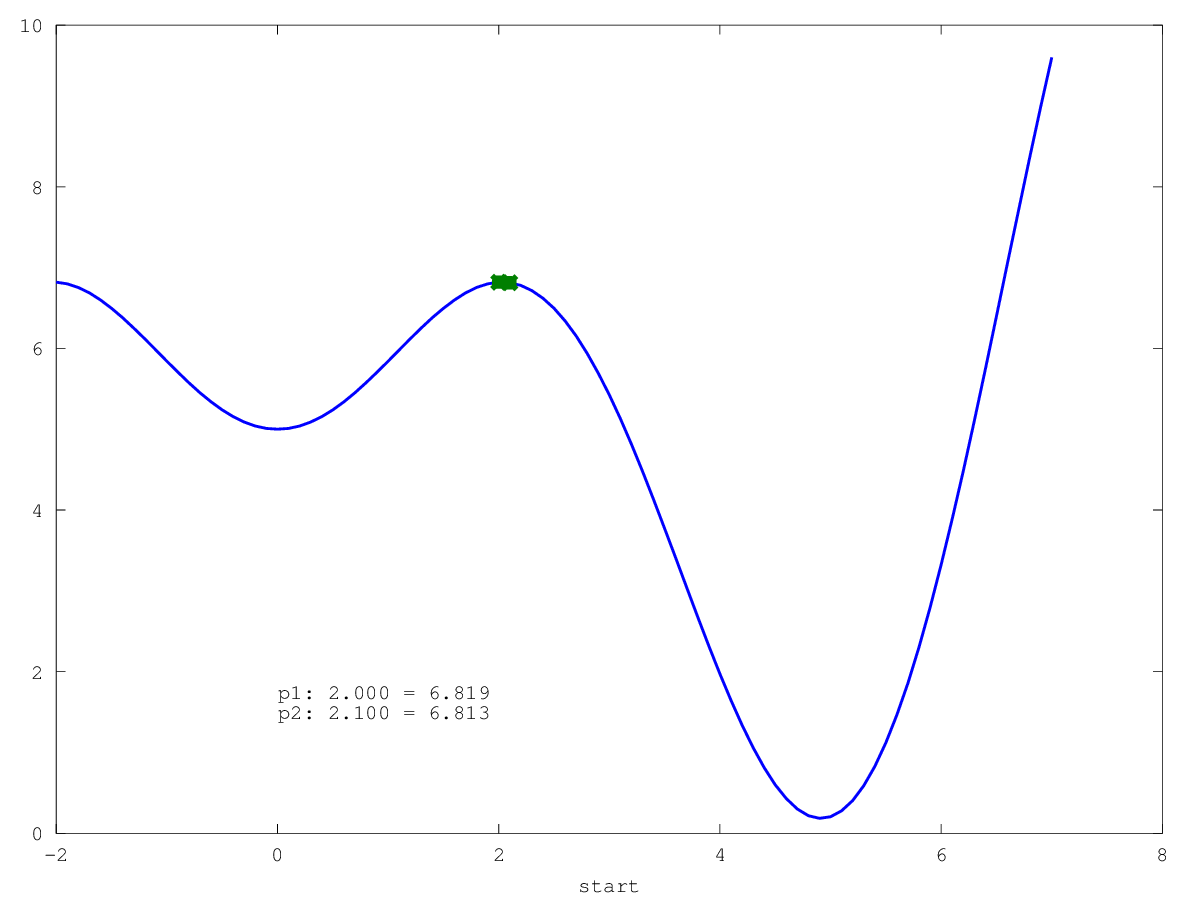
\includegraphics[width=\textwidth]{downhill/glob_sinx_x001.png}
\caption{Startsimplex}
\end{subfigure} \begin{subfigure}[b]{0.49\textwidth}
\centering
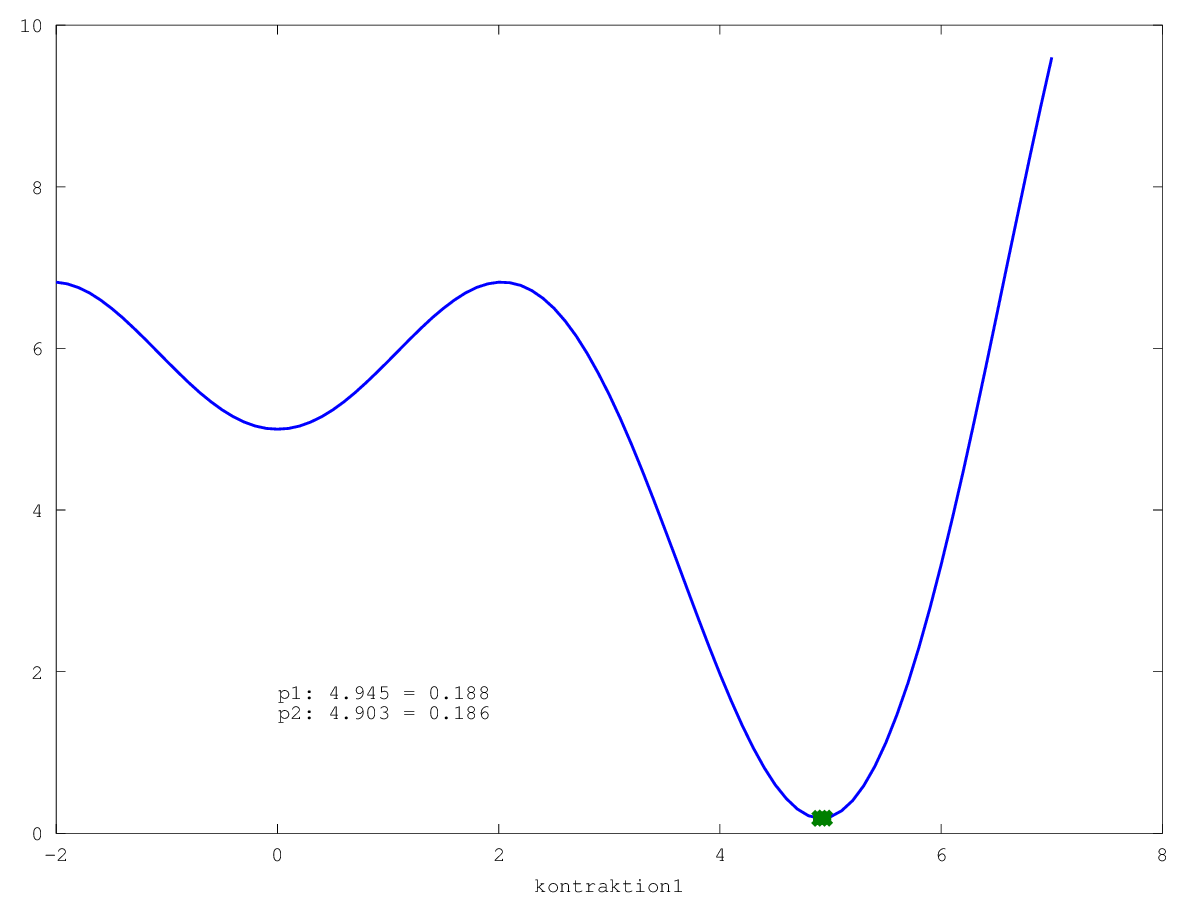
\includegraphics[width=\textwidth]{downhill/glob_sinx_x010.png}
\caption{Abbruch mit globalem Minimum}
\end{subfigure}
\caption{Globales Minimum}
\label{fig:downhillGlobMinima}
\end{figure}


\begin{figure}[htb]
\centering
\begin{subfigure}[b]{0.49\textwidth}
\centering
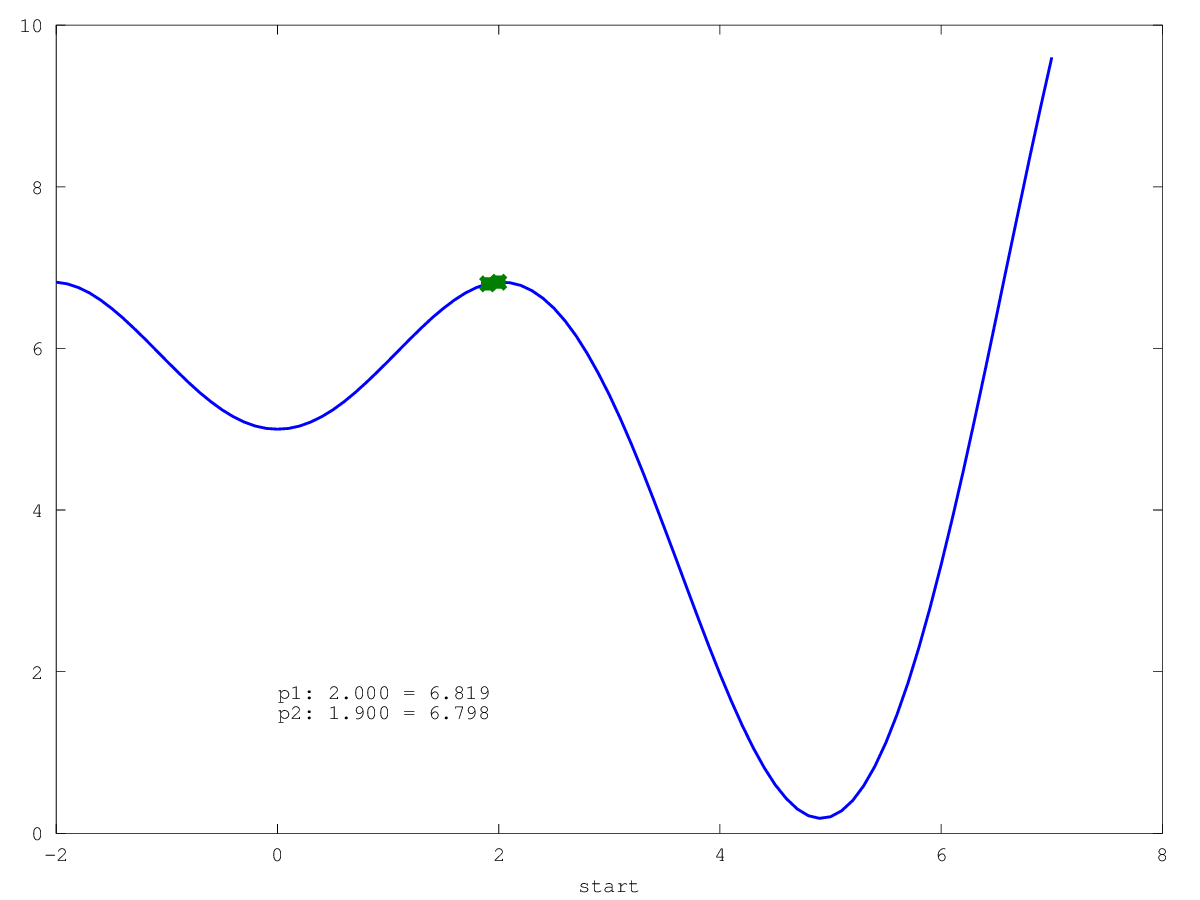
\includegraphics[width=\textwidth]{downhill/lok_sinx_x001.png}
\caption{Startsimplex}
\end{subfigure} \begin{subfigure}[b]{0.49\textwidth}
\centering
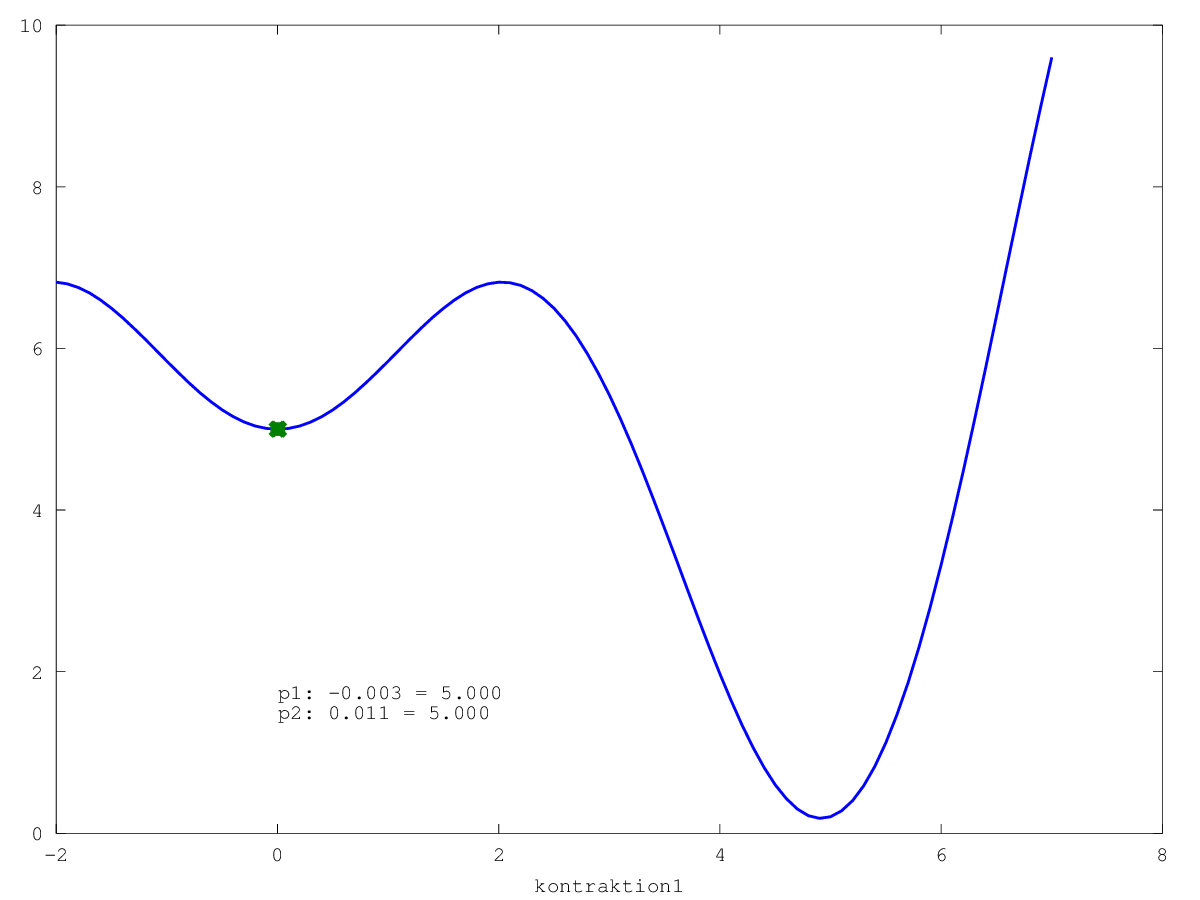
\includegraphics[width=\textwidth]{downhill/lok_sinx_x010.png}
\caption{Abbruch mit lokalem Minimum}
\end{subfigure}

\caption{Lokales Minimum}
\label{fig:downhillLokMinima}
\end{figure}

In \figref{fig:downhillGlobMinima} sieht man wie bei gut gew"ahltem Startsimplex der Algorithmus im globalen Minimum konvergiert.\\
Hingegen in \figref{fig:downhillLokMinima} konvergiert er auf ein lokales Minimum.


\subsubsection{Fr"uhzeitiges Zusammenziehen}
\label{sec:downhillZusammenziehen}
Der Algorithmus kann sich bei schlecht gew"ahltem Startsimplex und oder Parametern fr"uhzeitig zusammenziehen ohne in einem Minimum zu sein.\\
Das kann verhindert werden indem man das Startsimplex "uber ein gr"osseres Gebiet aufspannt oder den Parameter $\beta$ gr"osser w"ahlt.


\begin{figure}[htb]
\centering
\begin{subfigure}[b]{0.49\textwidth}
\centering
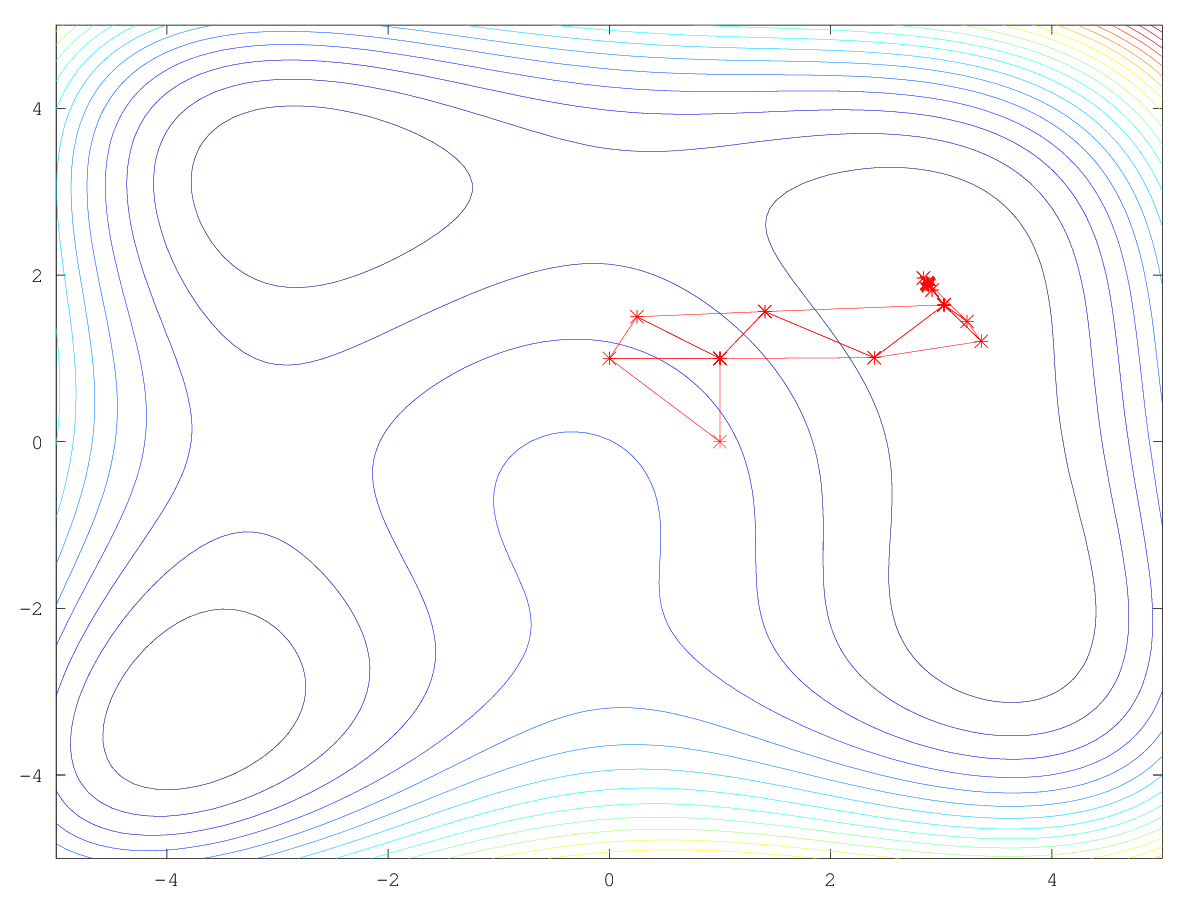
\includegraphics[width=\textwidth]{downhill/himmelblaubad.png}
\caption{Schlecht gew"ahlte Parameter: $z=0.967$}
\end{subfigure} \begin{subfigure}[b]{0.49\textwidth}
\centering
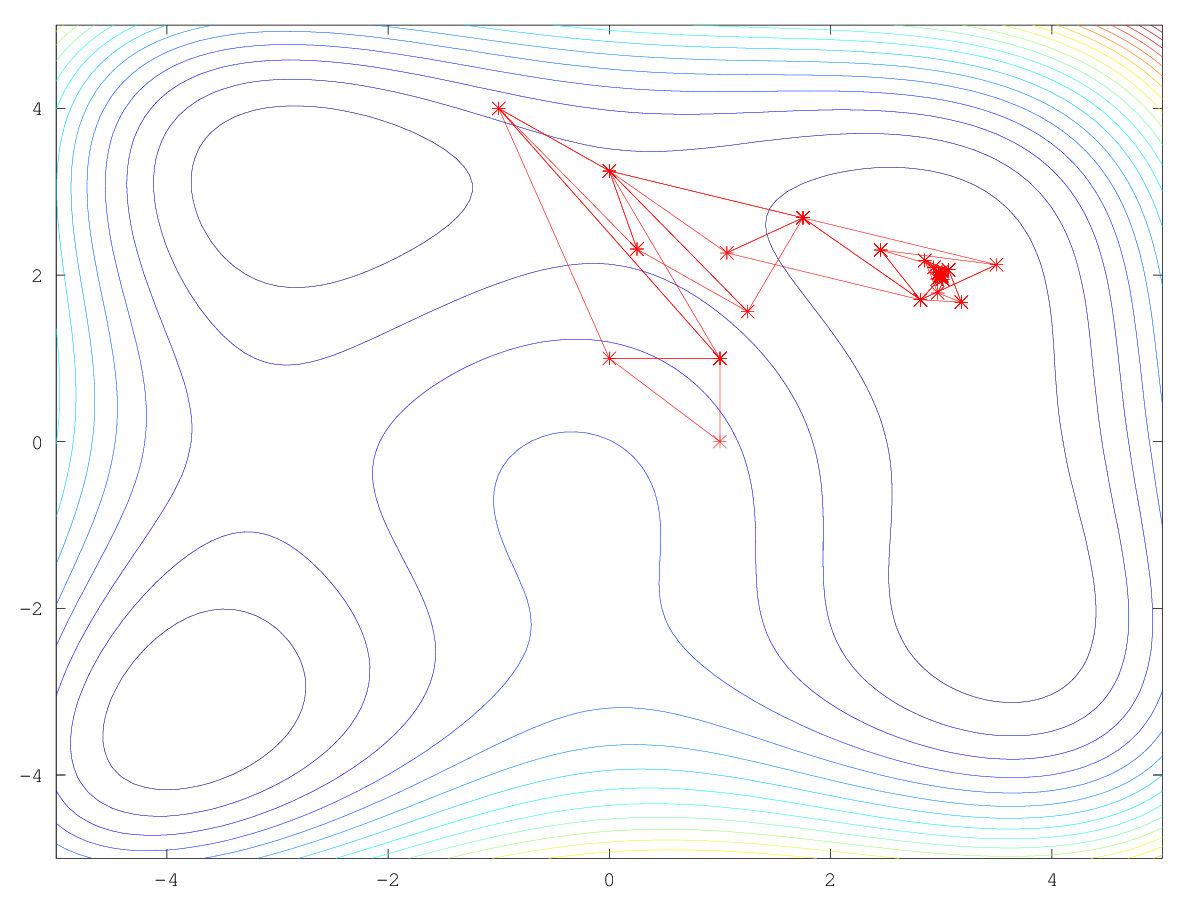
\includegraphics[width=\textwidth]{downhill/himmelblaugood.png}
\caption{Gut gew"ahlte Parameter: $z=0.000$}
\end{subfigure}

\caption{Simplex Verlauf "uber Himmelblau Funktion}
\label{fig:downhillHimmelblau}
\end{figure}
